\documentclass{article}

\usepackage[margin=50pt]{geometry}
\usepackage{placeins}
\usepackage{amsmath}
\usepackage{mathtools}
\usepackage{array,amsfonts}
\usepackage{amssymb}
\usepackage{physics}
\usepackage{graphicx}
\usepackage{subcaption}
\usepackage{anyfontsize}
\usepackage{enumitem}
\usepackage{etoolbox}
\usepackage[T1]{fontenc}
\usepackage[utf8]{inputenc}
\usepackage[english]{babel}
\usepackage{listings}
\usepackage[dvipsnames]{xcolor}
\usepackage[useregional]{datetime2}
\usepackage{glossaries}
\usepackage{xurl}
\usepackage[super]{nth}
\usepackage{hyperref}
\hypersetup{
    colorlinks=true,
    linktoc=all,
    linkcolor=blue,
}
\usepackage{fancyhdr}
    \pagestyle{fancy}
    \lhead{ML4G}
    \rhead{Kolly Florian}
    \renewcommand{\footrulewidth}{0.4pt}
    \renewcommand{\headrulewidth}{0.4pt}

\DeclareMathOperator{\sgn}{sgn}
\DeclareMathOperator{\Inf}{Inf}
\DeclareMathOperator{\Sup}{Sup}

\definecolor{def}{RGB}{79,129,189}
\definecolor{signif}{RGB}{118,146,60}
\definecolor{codegreen}{rgb}{0,0.6,0}
\definecolor{codegray}{rgb}{0.5,0.5,0.5}
\definecolor{codepurple}{rgb}{0.58,0,0.82}
\definecolor{backcolour}{rgb}{0.95,0.95,0.92}

\lstdefinestyle{pythonstyle}{
    backgroundcolor=\color{backcolour},
    commentstyle=\color{codegreen},
    keywordstyle=\color{magenta},
    numberstyle=\tiny\color{codegray},
    stringstyle=\color{codepurple},
    basicstyle=\ttfamily\footnotesize,
    breakatwhitespace=false,
    breaklines=true,
    captionpos=b,
    keepspaces=true,
    numbers=left,
    numbersep=5pt,
    showspaces=false,
    showstringspaces=false,
    showtabs=false,
    tabsize=2
}
\lstset{style=pythonstyle}

\apptocmd{\lim}{\limits}{}{}
\newcommand{\Z}{\mathbb{Z}}
\newcommand{\N}{\mathbb{N}}
\newcommand{\Q}{\mathbb{Q}}
\newcommand{\R}{\mathbb{R}}
\newcommand{\C}{\mathbb{C}}

\renewcommand{\phi}{\varphi}
\renewcommand{\epsilon}{\varepsilon}

\makeglossaries

\newglossaryentry{GIL}{name=GIL,description={Lock that allows only one thread to hold the control of the interpreter}}
\newglossaryentry{multithreading}{name=multithreading,description={A single processor execute multiple threads concurrently}}
\newglossaryentry{multiprocessing}{name=multiprocessing,description={Multiple processors run concurrently, where each processor can run one or more threads}}
\newglossaryentry{GAS}{name={GAS},description={for Gradient Accumulation steps, mechanism to split the batch of samples into mini-batches that run sequentially and that will add its gradient up to a total gradient}}
\newglossaryentry{SOTA}{name={SOTA},description={for State Of The Art, refers to the best models , in a specific subdomain or generally}}
\newglossaryentry{GPU}{name={GPU},description={for Graphics Processing Unit, is a specialized electronic circuit capable of computing matrix operations very quickly due to its parallel structure. It is used mostly in computer graphics, image processing and artificial intelligence}}
\newglossaryentry{TPU}{name={TPU},description={for Tensor Processing Unit, is a specialized integrated circuit for neural network machine learning}}

\makeglossaries

\begin{document}

\begin{titlepage}
  \begin{center}
    \Huge
    \textbf{\textcolor{def}{Data Parallelism in PyTorch}}
    \vspace{0.9cm}

    \LARGE
    ML4G - Project

    \vspace{1.9cm}
    \Large
    \textbf{\emph{Kolly Florian}}
    \vspace{5cm}
  \end{center}
  Version 0.5 (\DTMnow) - draft for alpha release
  \begin{center}
    \vspace{5cm}
    
\includegraphics[width=0.4\textwidth]{images/pytorch-logo.png}
    \vspace{10cm}
  \end{center}
\end{titlepage}

\setlength{\parindent}{0em}
\setlength{\parskip}{0.2em}

\tableofcontents
\newpage

\section{Disclaimer}
This document is heavily based on the available documentation online, that is the \href{https://pytorch.org/docs/stable/index.html}{officiel PyTorch documentation}, the \href{https://huggingface.co/docs}{Huggingsface documentation} and many others. All drawings are made with \href{https://www.draw.io}{draw.io}.

All mistakes are my own, and no warranty is given about the content and code in this document. Some examples of code are given and briefly described in the annex section of this document. The Python version used here is 3.6. Please understand that this document started as and still is a personal documentation and is not written by an expert, nor a professional writer.

The author would like to thank the ML4G organizers and the EffiSciences team behind for the camp where this document began, and especially Charbel-Raphael and Quentin for their advices and the great exchanges I had with them. A huge thank to my friend Leo Meier for spending a long night helping me with some diagrams and for her continued support, and to my all my other friends at EPFL for listening to me trying to explain parallelization, hopefully with a bit of success.

ALPHA RELEASE DISCLAIMER: This version is an alpha release, not intended for public access. Multiple reviews and rewritings can and will be made on any section of this document. Many chapters, if not most, are incomplete and/or deserve more clarity. The author is aware of those issues.

\section{For whom is this document written?}
For anyone who wants to get started in developing parallelized models with PyTorch! More precisely, the reader should have familiarity with PyTorch and knowledge on how to build simple models. Most of the examples here won't include important parts of the code (e.g. the training loop), the reader is expected to be able to fill these gaps.

\clearpage

\section{Introduction to Data Parallelism}
Data parallelism is a technical concept referring to scenarii in which an operation is concurrently performed on elements in a source collection. The goal is to partition the source so that multiple processes can compute on different segments at the same time. Nowadays, we mostly use \GLS{GPU}s and \GLS{TPU}s to parallelize operations. There are two major motivations for which one wants to implement data parallelism:
\begin{itemize}
  \item Firstly, today's models are too voluminous to be stored on a single \GLS{GPU}. Note that this trend is (at the time of writing) not slowing down, we thus expect \Gls{SOTA} models to get even bigger in the near future
  \item Secondly, we crave speed. While a model might take years to run on a single \GLS{GPU} (or a single machine), we want it to run in a matter of hours
\end{itemize}

\subsection{First, a bit of terminology}
All across this documentation and most of the ones you can find online, a few terms will often come back. Let's explain them briefly here (we will come back to them later in more details).

\begin{itemize}
  \item \textbf{World}: term used to describe all the processing units available, not depending on which device they run nor which process they are handling. The \textbf{world size} refers to the total number of processing unit
  \item \textbf{Node}: name of a device that is connected to a specific communication group
  \item \textbf{Rank}: unique ID given to a processing unit
  \item \textbf{Local rank}: same as the rank, but on a specific node
  \item \textbf{Root}: specific process considered as the main one. It is usually given rank 0, but this is no obligation
\end{itemize}
For clarity, consider the following example:
\begin{figure}[h!]
  \center
  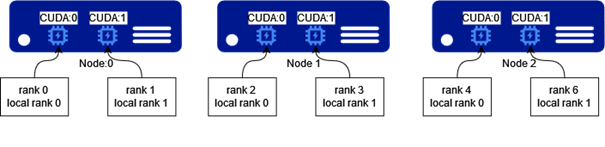
\includegraphics[width=0.7\linewidth]{images/2022-08-24-17-37-31.png}
  \caption{Take some time to compare the rank and the local rank}
\end{figure}
\FloatBarrier

We have three different devices (thus 3 nodes) that each contains 2 \GLS{GPU}s. All of them combined give us the world, with a world size of 6. Notice how the rank is a unique number across the entire world.

\subsection{Type of parallelization}
We can distinguish between different types or methods of parallelization: whether we parallelize the data, the tensors or the models. We will later come back to each method in much more detail.
\begin{itemize}
  \item Model Parallelism (MP): the model is split up across multiple \GLS{GPU}s. We split along the layers, or group of layers, and each \GLS{GPU} handles a specific block.
  \item Data Parallelism (DP): the same program is replicated multiple times on multiple devices, and each device is being fed a slice of the data. We synchronize the devices at the end of each training step.
  \item Tensor Parallelism (TP): each tensor is split up into multiple chunks, residing separately on a designated \GLS{GPU}. After each shard gets processed separately, the results are synced together.
  \item Pipeline Parallelism (PP): the model is split up across multiple \GLS{GPU}s. Each \GLS{GPU} processes in parallel different stages of the pipeline on a small chunk of the batch.
  \item Zero Redundancy Optimizer (ZeRO): somewhat similar to Tensor Parallelism, except that the whole tensor gets reconstructed in time for a forward or backward computation (no modification on the model). We will come back to this technique later in more details, as it is a quite revolutionary technology.
\end{itemize}

Another way to distinguish between types of parallelism is called the Flynn's taxonomy. It is a more generic classification based on the number of concurrent instruction and data streams:
\begin{itemize}
  \item SISD (Single Instruction Single Data): single uniprocessor machine that can execute a single instruction and fetch single data stream from memory
  \item SIMD (Single Instruction Multiple Data): a device that can issue the same single instruction to multiple data simultaneously (e.g. \GLS{GPU})
  \item MISD (Multiple Instruction Single Data): architecture used for fault tolerance, where several systems act on the same data and must agree (we won't talk about it here)
  \item MIMD (Multiple Instruction Multiple Data): multiple processors executing different instruction on different data (distributed systems)
  \item SPMD (Single Program Multiple Data): single program executed by a multi-processor device or cluster of devices
  \item MPMD (Multiple Program Multiple Data): multiple programs executed by multi-processor device or cluster of devices
\end{itemize}

\subsubsection{Model Parallelism (MP)}
Also called vertical data parallelization, the idea of model parallelism is to spread layers or groups of layers across multiple \GLS{GPU}s. In PyTorch, this is done by moving the layers (and data right before it reaches the layer) with the \lstinline{.to()} method to the desired device.
\begin{figure}[h!]
  \center
  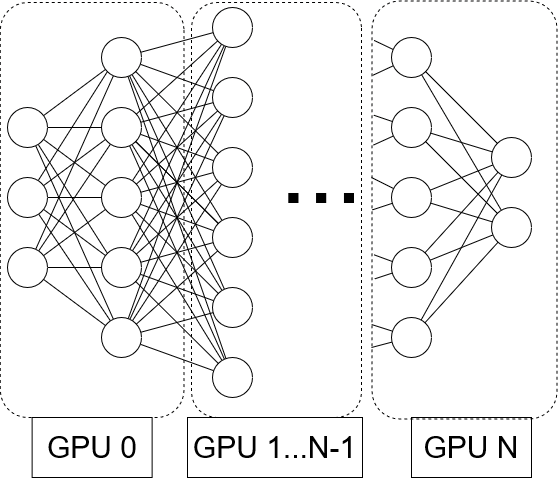
\includegraphics[width=0.5\linewidth]{images/2022-08-24-18-23-26.png}
  \caption{We split our models vertically, separating groups of layers in multiple \GLS{GPU}s}
\end{figure}
\FloatBarrier
Note that there is an information overhead when the data transit from one \GLS{GPU} to another, especially if the \GLS{GPU}s are not on the same node. Moreover, to be able to compute the loss, we often need to send the data back to the first layer where the labels are once the last layer is done.

The main advantage of model parallelism is that it allows for bigger model to be trained, as the \GLS{GPU}s share the memory load. However, all but one \GLS{GPU} is idle at any given time and it has an overhead of copying the data between the devices (especially if they are not on the same node). Remark that it is better to have a 24GB card instead of 4x6GB cards using this parallelism paradigm.

\subsubsection{Pipeline parallelism (PP)}
This technique is very similar to the previous one, except that we artificially introduce a pipeline to use all \GLS{GPU}s concurrently. Let's compare a typical forward and backward pass. First, here is the flow for a simple model parallelism:

\begin{figure}[h!]
  \center
  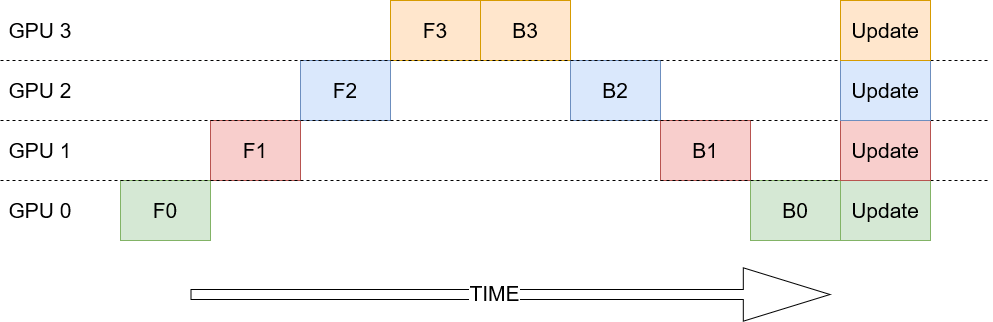
\includegraphics[width=0.7\linewidth]{images/2022-08-25-09-22-17.png}
  \caption{Notice the poor use of each \GLS{GPU}}
\end{figure}
\FloatBarrier

Pipeline parallelism creates mini-batches of data to keep most of the \GLS{GPU}s running most of the time.

\begin{figure}[h!]
  \center
  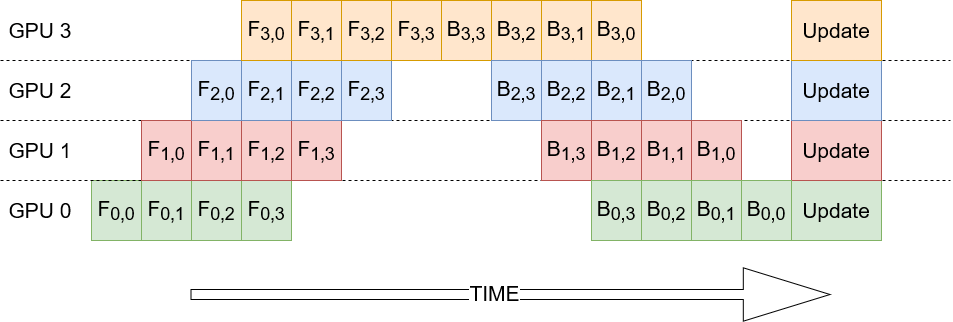
\includegraphics[width=0.7\linewidth]{images/2022-08-25-09-22-51.png}
  \caption{This is much better. Take a moment to look at the indices!}
\end{figure}
\FloatBarrier

The idle parts are referred to as the "bubble". This method introduces a new parameter, the \textit{chunks}, that define how many chunks of data are sent in a sequence through the same pipe stage (the chunk is 4 in the image above). Adding a layer of data parallelism over the pipeline parallelism, we need to distinguish between mini-batches and micro-batches. The global data is first split into mini-batches as usual (e.g. a batch size of 1024 gets split up into 4 mini-batches of 256 each). The pipeline then splits each mini-batches by the number of chucks to obtain a micro-batch (e.g. 32 chunks yield micro-batches of size 8, continuing on the example above). Each stage works with a single micro-batch at a time. One needs to be careful when choosing those sizes: too small and the \GLS{GPU}s won't be used enough, too big and the micro-batches become too tiny.

\subsubsection{Tensor parallelism (TP)}
In tensor parallelism, each \GLS{GPU} processes only a slice of a tensor. The full tensor is aggregated only for operations that require it as a whole unit. Let's take a quick detour through linear algebra to better understand it.

If we have two matrices for which we want to find the dot product, it is possible to split either column-wise or row-wise. For example, the following product

\[\underbrace{\begin{pmatrix}
0 & 1 & 2 & 3\\
4 & 5 & 6 & 7
\end{pmatrix}}_{A}\cdot \underbrace{\begin{pmatrix}
8 & 9\\
10 & 11\\
12 & 13\\
14 & 15
\end{pmatrix}}_{B}=\underbrace{\begin{pmatrix}
76 & 82\\
252 & 274
\end{pmatrix}}_{Y}\]

can also be done splitting matrix B column-wise:

\begin{gather*}
  Y_1=\begin{pmatrix}
    0 & 1 & 2 & 3\\
    4 & 5 & 6 & 7
    \end{pmatrix}\cdot \begin{pmatrix}8\\10\\12\\14\end{pmatrix}
    =\begin{pmatrix}76\\252\end{pmatrix} \\
    Y_2=\begin{pmatrix}
      0 & 1 & 2 & 3\\
      4 & 5 & 6 & 7
      \end{pmatrix}\cdot \begin{pmatrix}9\\11\\13\\15\end{pmatrix}
      =\begin{pmatrix}82\\274\end{pmatrix} \\
      Y=Y_1 \mathbin\Vert Y_2
\end{gather*}

and by splitting matrix \(A\) by rows and matrix \(B\) by columns before summing the results:

\begin{gather*}
  Y_1=\begin{pmatrix}0 & 1\\4 & 5\end{pmatrix}\cdot \begin{pmatrix}8 & 9\\10 & 11\end{pmatrix}
  =\begin{pmatrix}10 & 11\\82 & 91\end{pmatrix} \\
  Y_2=\begin{pmatrix}2 & 3\\6 & 7\end{pmatrix}\cdot \begin{pmatrix}12 & 13\\14 & 15\end{pmatrix}
  =\begin{pmatrix}66 & 71\\170 & 183\end{pmatrix} \\
  Y=Y_1+Y_2
\end{gather*}

Using these techniques, we can then split a weight matrix \(A\) column-wise across \(N\) \GLS{GPU}s and perform the matrix multiplications in parallel. It is also possible to feed them into an activation function independently.

\begin{figure}[h!]
  \center
  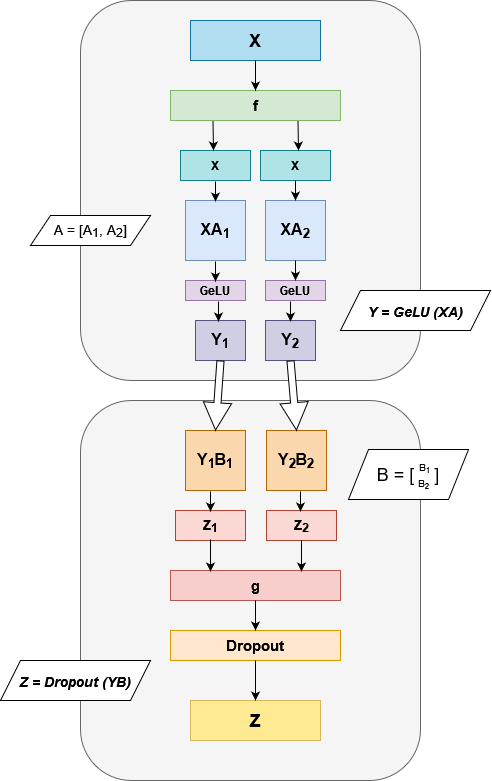
\includegraphics[width=0.4\linewidth]{images/2022-08-25-10-04-26.png}
  \caption{Example of tensor parallelism, through the activation function}
\end{figure}
\FloatBarrier

We need to synchronize only at the end, where the output vector has to be reconstructed.

One major issue unfortunately is that tensor parallelism requires a fast transfer of data. It is thus not advisable to do tensor parallelism over more than one node (i.e. device).

\subsubsection{Combinations}
There are many ways to combine the parallelism tools seen above. Some will be detailed in greater details later. Usually, these methods are implemented by known frameworks such as DeepSpeed, Megatron-LM, SageMaker or OSLO.

\subsubsection{Which methods should I use?}
It is almost impossible to give a straight answer, as the best techniques to use will always depend on many factors such as the size of the model, the compute time available, the compute ressources at disposition and of course the price one is willing to pay to train his model. However, here are a few guidelines:
\begin{itemize}
  \item Single \GLS{GPU}
  \begin{enumerate}
    \item Model fits onto a single \GLS{GPU}: no parallelization necessary
    \item Model doesn't fit onto a single \GLS{GPU}: ZeRO + Offload CPU
    \item Largest layer doesn't fit into a single \GLS{GPU}: Memory Centric Tiling*
  \end{enumerate}
  \item Single Node / Multi-\GLS{GPU}
  \begin{enumerate}
    \item Model fits onto a single \GLS{GPU}: Distributed DP / ZeRO
    \item Model doesn't fit onto a single \GLS{GPU}: PP / ZeRO / TP
    \item Largest layer doesn't fit into a single \GLS{GPU}: ZeRO / TP
  \end{enumerate}
  \item Multi-node / Multi-\GLS{GPU}
  \begin{enumerate}
    \item ZeRO (simplest) / PP+TP+DP (massive changes to the model)
  \end{enumerate}
\end{itemize}

* Memory Centric Tiling allows to run arbitrarily large layers by automatically splitting them and executing them sequentially.

\subsection{Parallelization in PyTorch}
In PyTorch, the \lstinline{torch.distributed} package contains much of the utilities necessary to begin working with parallelized systems. The official documentation categorizes the package into three main components:
\begin{itemize}
  \item Distributed Data-Parallel Training (DDP): the model is replicated on every process and every model replica will be fed with a different set of input data. The gradient is synchronized on every replicas, along with its computation to speed up the process.
  \item RPC-Based Distributed Training (RPC): RPC supports training structures such as distributed pipeline parallelism, parameter sever paradigm for examples. Its main avantage is the extension of the autograd engine beyond machine-boundaries.
  \item Collective Communication (c10d): this library is the API on which DDP and RPC are built (resp. collective communication and P2P). It allows for finer-grain control over what is communicated between the replicas but in exchange gives up the performance optimizations.
\end{itemize}

\subsubsection{Data Parallel Training Paradigm}
When working on projects that are expected to gradually grow in complexity, a common development strategy is as follows:
\begin{enumerate}
  \item Single-machine single-\GLS{GPU} training: default behaviour
  \item Single-machine multi-\GLS{GPU} training: DataParallel module
  \item Single-machine multi-\GLS{GPU} distributed training: DistributedDataParallel module
  \item Multi-machine multi-\GLS{GPU} distributed training: DistributedDataParallel module, additional scripting required
  \item Dynamic multi-machine multi-\GLS{GPU} distributed training: elastic package
\end{enumerate}

\section{Data-Parallel Training}
\lstinline{nn.parallel.DataParallel} is the simplest package to allow parallelism during the training process, as it requires only minor additional code (one line is often enough). However, it does not offer the best performances as it replicates the model in every forward pass. The major issue is that it is a single-process multi-thread parallelism that bounds the speed due the infamous \Gls{GIL} single-lock.

\subsection{Using DP on a model}
The package \lstinline{DataParallel} handles everything on its own. To allow data parallelization on a model in PyTorch, one must simply tell PyTorch to use the module on a given model. We can also indicate which devices to use using the \lstinline{device_ids} parameter:

\begin{lstlisting}[language=Python]
model = nn.DataParallel(model, device_ids=[0,1])
\end{lstlisting}

\section{Distributed Data-Parallel Training}
While being harder to setup and use, the package \lstinline{nn.parallel.DistributedDataParallel} is a far more common choice than simply using \lstinline{nn.parallel.DataParallel}. This is due to two main advantages of \lstinline{DistributedDataParallel}:
\begin{itemize}
  \item Each process maintains its own optimizer and performs a complete optimization step with each iteration. Thus, no parameter broadcast step is needed, reducing the tensors transfer time
  \item Each process contains an independent Python interpreter, thus avoiding the GIL single-lock and making heavy use of the Python runtime
\end{itemize}

The second advantage is that \lstinline{dataParallel} is \gls{multithreading} while \lstinline{distributedDataParallel} is \gls{multiprocessing}. This can and does make a huge difference in Python.

\subsection{Understanding the backends}
The \lstinline{torch.distributed} package supports three built-in backends that allow the transport of data across multiple processes and/or nodes. This part is important only for readers who want or need to dig deeper into the parallelism world, and can be skipped otherwise.

\subsubsection{MPI}
MPI (Message Passing Interface) is a library standard for programming distributed memory. MPI is portable and fast, as it has been implemented and optimized on almost all architectures and hardwares. It has language bindings for Fortran, C and C++ and several MPI modules exist in Python.

MPI model consists of communications among processes through messages called \textit{inter-process communication}. All the nodes execute the same program but each have a unique ID (rank), allowing the user to select which part should be executed by which process. This is very important to understand: the program is the same across the nodes! To ask a specific device to go through a part of the code, one can use its rank in a condition before.

\begin{figure}[h!]
  \center
  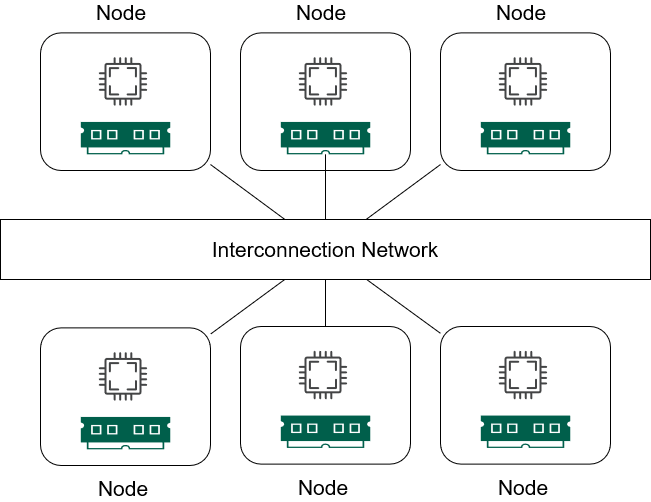
\includegraphics[width=0.5\linewidth]{images/2022-08-25-11-00-37.png}
  \caption{Multiple nodes, each with a compute capabilities and memory, are linked by an interconnection network}
\end{figure}
\FloatBarrier

\paragraph{MPI Communicator}
An MPI communicator is a "communication universe" for a group of processes. The default MPI communicator is called \lstinline{MPI_COMM_WORLD} and represents the collection of all processes. Almost every MPI command needs to provide a communicator as argument.

\paragraph{Handling the process rank}
As seen at the beginning, a rank is used to distinguish a process from the others: it is a unique integer value assigned to a process within a communicator. Here is a classical way to setup and use ranks with MPI (in C):
\begin{lstlisting}[language=C]
int size, rank;
MPI_Comm_size(MPI_COMM_WORLD, &size);
MPI_Comm_rank(MPI_COMM_WORLD, &rank);
// The root node has usually rank 0
if(rank == 0) {...}
\end{lstlisting}

\paragraph{Initiating and closing a computation}
Among the most important MPI commands are those used for initiating and closing a computation:
\begin{lstlisting}[language=C]
int main(int argc, char** argv) {
  MPI_Init(&argc, &argv); // initiates an MPI computation
  ...
  MPI_Finalize(); // terminates the MPI computation and cleans up
}
\end{lstlisting}

\paragraph{Synchronization}
Often, parallel algorithms require that no process continues on before all the processes have reached a certain state at certains points in the program. For that, it is possible to ask for explicit synchronization:
\begin{lstlisting}[language=C]
int MPI_Barrier(MPI_Comm comm);
\end{lstlisting}

\paragraph{Blocking communication}
In MPI, communication consists of sending a copy of the data to another process. On the sender side, the communication requires to know the rank of the receiver, the data type, the size and the location where the message needs to be sent. The receiver does \textit{not} need to know who the sender is, but only the data type, size and what storage location to use to put the resulting message.

More strictly speaking, MPI defines a function that performs blocking send:
\begin{lstlisting}[language=C]
int MPI_Send(const void *buf, int count, MPI_Datatype datatype, int dest, int tag, MPI_Comm comm)
\end{lstlisting}
where \lstinline{buf}, \lstinline{count} and \lstinline{datatype} define the message buffer (the \textit{data}), \lstinline{dest} and \lstinline{comm} identify the destination process. The \lstinline{tag} parameter is optional. The last three described are collectively called the \textit{envelope} The message gets sent and the buffer empties out before the function exits.
On the other end, a function performs a blocking receive:
\begin{lstlisting}[language=C]
int MPI_Recv(void *buf, int count, MPI_Datatype datatype, int source, int tag, MPI_Comm comm, MPI_Status *status)
\end{lstlisting}
This function waits for a message from \lstinline{source} and \lstinline{comm} and once received stores it into the buffer defined by \lstinline{buf}, \lstinline{count} and \lstinline{datatype}. One can used \lstinline{MPI_ANY_SOURCE} to receive from any source and/or \lstinline{MPI_ANY_TAG} to receive from any tag. Note that receiving fewer \lstinline{datatype} elements than \lstinline{count} is fine, but receiving more results in an error. The \lstinline{status} is a useful structure that contains information about (for example) the source (\lstinline{status.MPI_SOURCE}) or the tag (\lstinline{status.MPI_TAG}).

\paragraph{Non-blocking communication}
Of course, non-blocking communications are also possible: the following methods return immediately, and the computation and communication can be overlapped:
\begin{lstlisting}[language=C]
int MPI_Isend(const void *buf, int count, MPI_Datatype datatype, int dest, int tag, MPI_Comm comm, MPI_Request *request)
int MPI_Irecv(void *buf, int count, MPI_Datatype datatype, int source, int tag, MPI_Comm comm, MPI_Request *request)
\end{lstlisting}

\paragraph{Collective communication}
Collective communication refers to the process of synchronizing and moving data or creating pool of collective computation. It involves all the processes within the scope of a communicator. By default, all the processes are in the \lstinline{MPI_COMM_WORLD} communicator, but it is possible to define groups of communicators.

\begin{itemize}
  \item Broadcasting: share data from the process with rank root to all other processes of the communicator including the root process
  \begin{lstlisting}[language=C]
int MPI_Bcast(void *buf, int count, MPI_Datatype datatype, int root, MPI_Comm comm)
  \end{lstlisting}
  \begin{figure}[h!]
    \center
    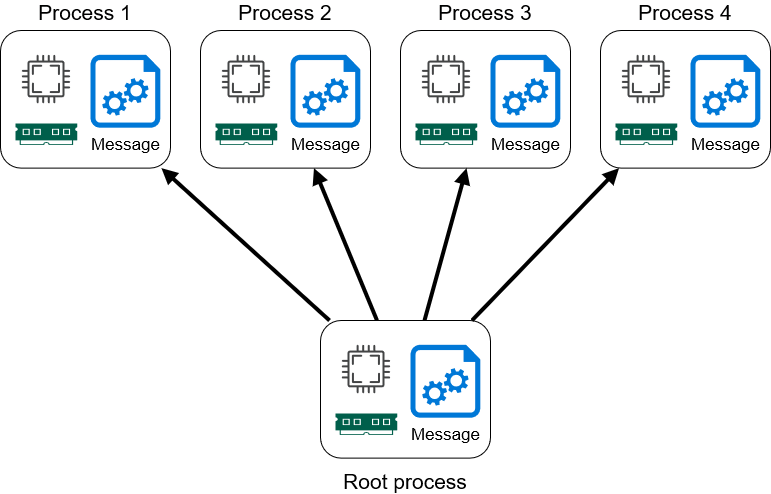
\includegraphics[width=0.65\linewidth]{images/2022-08-30-13-54-28.png}
    \caption{Broadcasting data}
  \end{figure}
  \FloatBarrier
  \item Scattering: send a fraction of data to each node
  \begin{lstlisting}[language=C]
int MPI_Scatter(const void *sendbuf, int sendcount, MPI_Datatype sendtype, void *recvbuf, int recvcount, MPI_Datatype recvtype, int root, MPI_Comm comm)
  \end{lstlisting}
  \begin{figure}[h!]
    \center
    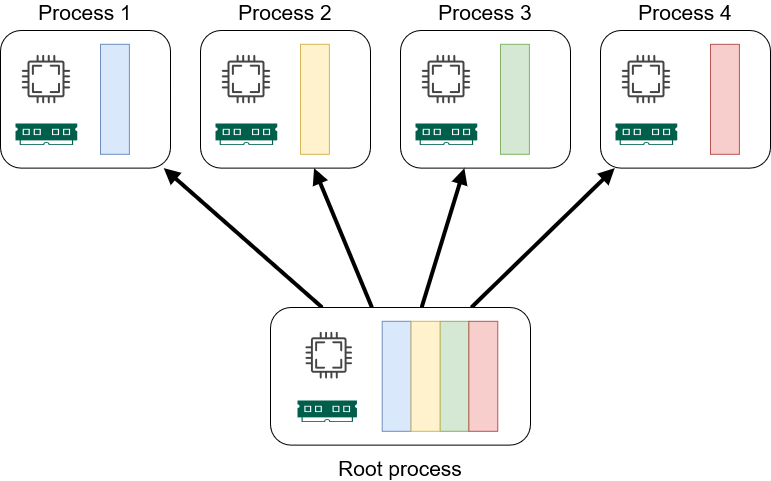
\includegraphics[width=0.65\linewidth]{images/2022-08-30-14-03-58.png}
    \caption{Scattering data}
  \end{figure}
  \FloatBarrier
  \item Gathering: retrieve a portion of data from different processes
  \begin{lstlisting}[language=C]
int MPI_Gather(const void *sendbuf, int sendcount, MPI_Datatype sendtype, void *recvbuf, int recvcount, MPI_Datatype recvtype, int root, MPI_Comm comm)
  \end{lstlisting}
  \begin{figure}[h!]
    \center
    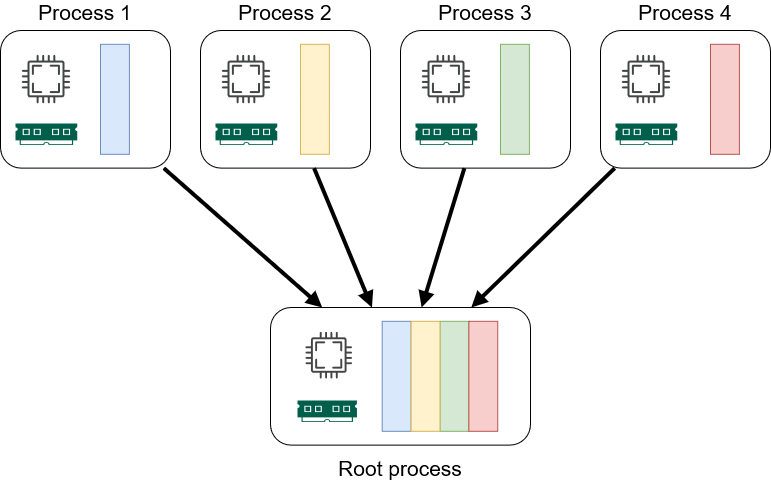
\includegraphics[width=0.65\linewidth]{images/2022-08-30-14-08-05.png}
    \caption{Gathering data}
  \end{figure}
  \FloatBarrier
  \item Reducing: retrieve a portion of data from different processes and manipulate it directly
  \begin{lstlisting}[language=C]
int MPI_Reduce(const void *sendbuf, void *recvbuf, int count, MPI_Datatype datatype, MPI_Op op, int root, MPI_Comm comm)
  \end{lstlisting}
  \begin{figure}[h!]
    \center
    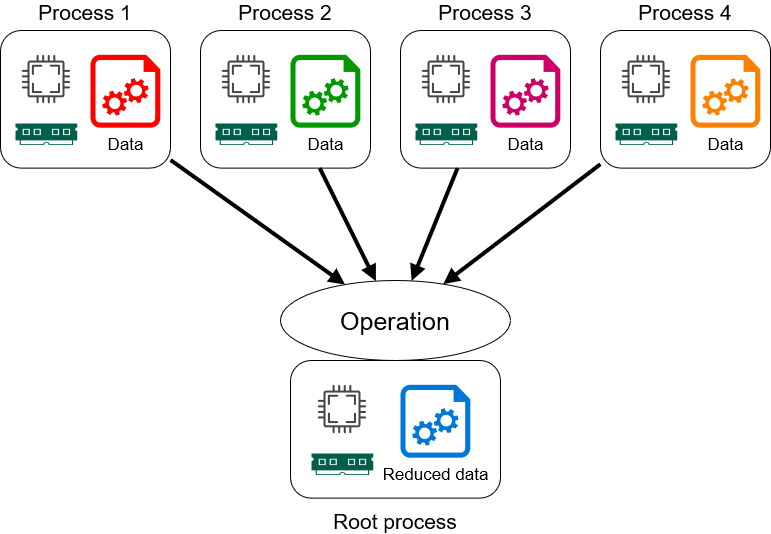
\includegraphics[width=0.65\linewidth]{images/2022-08-30-14-16-20.png}
    \caption{Reducing data}
  \end{figure}
  \FloatBarrier
\end{itemize}

\subsubsection{NCCL}
NCCL (for NVIDIA Collective Communications Library, pronounced "Nickel") is a library providing inter-\GLS{GPU} communication functions (called primitives). Like MPI, it implements both point-to-point send/receive and collective communication primitives. However, contrary to MPI, it is not a parallel programming framework, but aims at accelerating inter-\GLS{GPU} communication. NCCL implements each collective communication primitives in a single kernel handling both communications and computation operations, allowing for fast synchronization and minimizing the resources needed to reach peak bandwidth. This tool works on any multi-\GLS{GPU} parallelization model (e.g. single-threaded control of all \GLS{GPU}s, multi-threaded (one thread per \GLS{GPU}), multi-process with MPI, ...).

NCCL possesses a C API, accessible from multiple programming languages and follows the MPI collectives API. The most important modification is the presence of a \lstinline{stream} argument providing direct integration with the CUDA programming model.

The collective communication primitives implemented by NCCL are the following:
\begin{itemize}
  \item AllReduce
  \item Broadcast (see MPI broadcast)
  \item Reduce (see MPI reduce)
  \item AllGather
  \item ReduceScatter
\end{itemize}

Let's draw the schema for the primitives that haven't been covered yet:

\begin{itemize}
  \item All reducing: same as reduce, but the result is stored in all processes
  \begin{figure}[h!]
    \center
    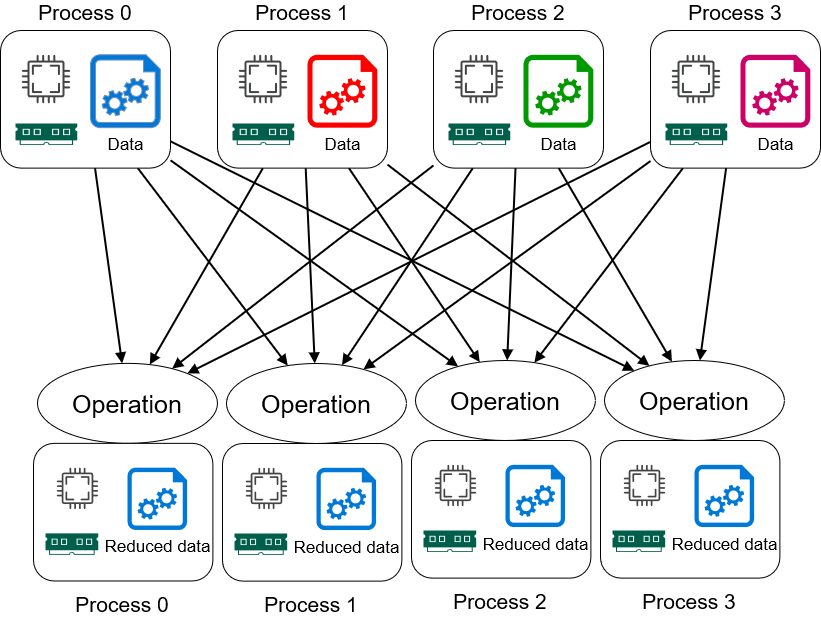
\includegraphics[width=0.65\linewidth]{images/2022-09-05-16-27-58.png}
    \caption{All reducing data}
  \end{figure}
\FloatBarrier
  \item All gathering: retrieve a portion of data from all processes to all processes
  \begin{figure}[h!]
    \center
    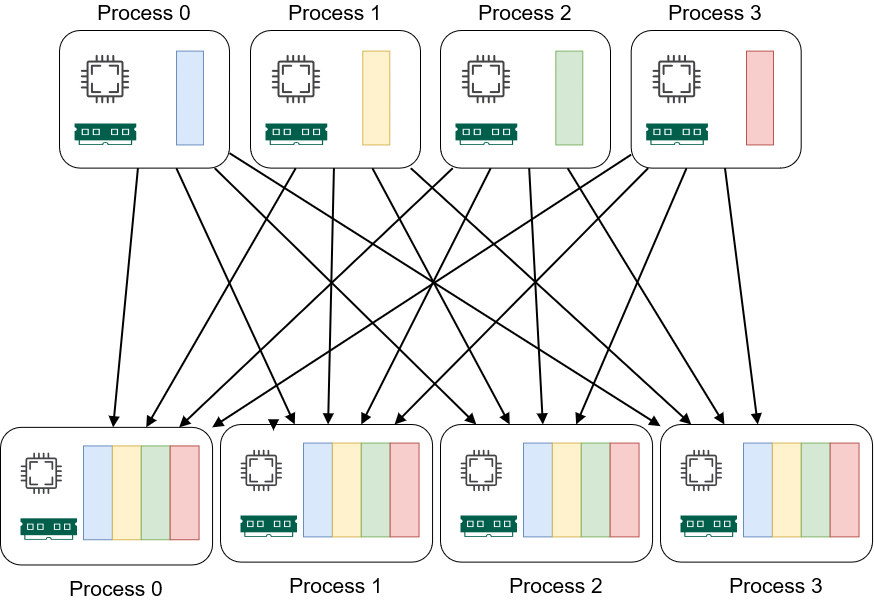
\includegraphics[width=0.65\linewidth]{images/2022-09-05-16-42-14.png}
    \caption{All gathering data}
  \end{figure}
  \FloatBarrier
  \item Reduce scattering: same as reduce, except the result is scattered in equal blocks among ranks
  \begin{figure}[h!]
    \center
    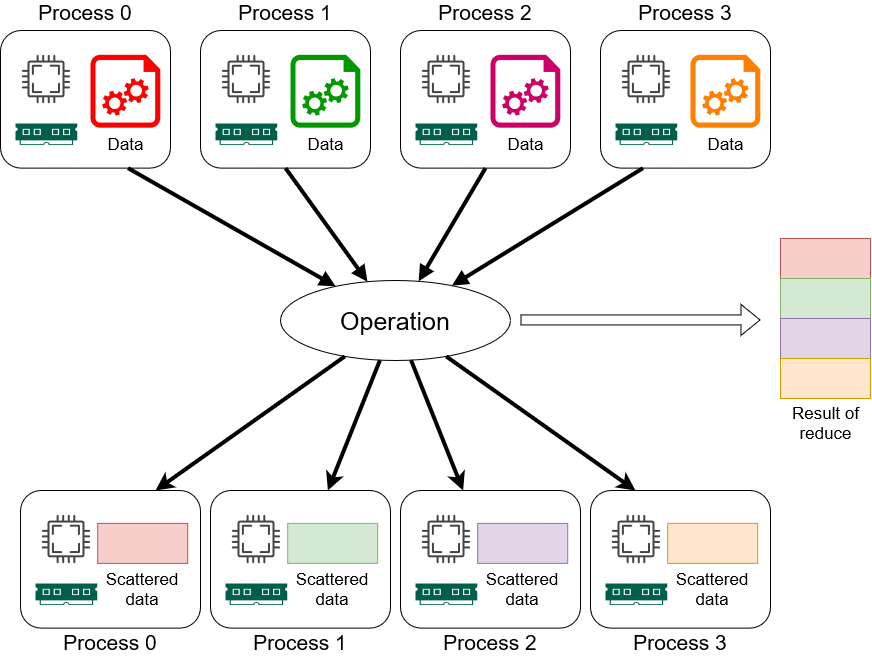
\includegraphics[width=0.65\linewidth]{images/2022-09-07-14-42-30.png}
    \caption{Reduce scattering data}
  \end{figure}
  \FloatBarrier
\end{itemize}

\paragraph{A bit more theory into how NCCL works}
NCCL is a topology-aware ring-based library, implemented as monolithic CUDA C++ kernels with three primitive operations (Copy, Reduce and ReduceAndCopy). Ring-based means that a \GLS{GPU} is connected to its following one, forming a ring-like structure:

\begin{figure}[h!]
  \center
  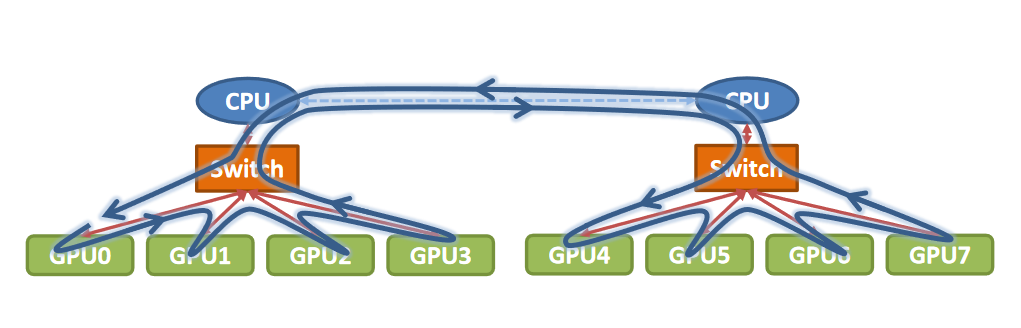
\includegraphics[width=0.75\linewidth]{images/2022-09-07-15-37-09.png}
  \caption{Example of a ring-based collective}
\end{figure}
\FloatBarrier

\subsubsection{Gloo}
Gloo is a collective communications library hosted by the Meta Incubator (yes, the same Meta as Facebook). Its library offers many distributed algorithms: when applicable, these algorithms have an implementation that works with system memory buffers, and one that works with Nvidia \GLS{GPU} memory buffers (using CUDA and NCCL). In the latter case, it is not necessary to copy memory between host and device.

The first thing the Gloo framework does is called the \emph{rendezvous}: the nodes find each other and setup connections between them (full mesh, i.e. bidirectional communication, or some subset). A \lstinline{gloo::Context} class retains information about all the participating processes (the ranks) and the persistent communication channels. Gloo does not maintain global state or thread-local state, meaning one can setup as many contexts as needed!

The algorithms available in Gloo are the following:
\begin{itemize}[noitemsep]
  \item AllReduce (see NCCL above)
  \item Reduce-Scatter (see NCCL above)
  \item Broadcast (see MPI above)
  \item pairwise\_exchange (see MPI above)
\end{itemize}

Note that it is possible to use an existing MPI communicator to create the \emph{rendezvous} context (key/value). Gloo won't use it after.

\subsubsection{Let's recap}
The last sections described the three backends usable with PyTorch (under certain conditions), that is MPI, NCCL and Gloo. Their implementation of the primitives can differ a lot, thus affecting the speed of computation. There is also a difference in what primitives are implemented. It is therefore impossible to tell the reader which one to use, it all falls down on the use case.

NVIDIA offers a great summary picture for their backend NCCL. You can also find some of the primitives of the other backends:

\begin{figure}[h!]
  \center
  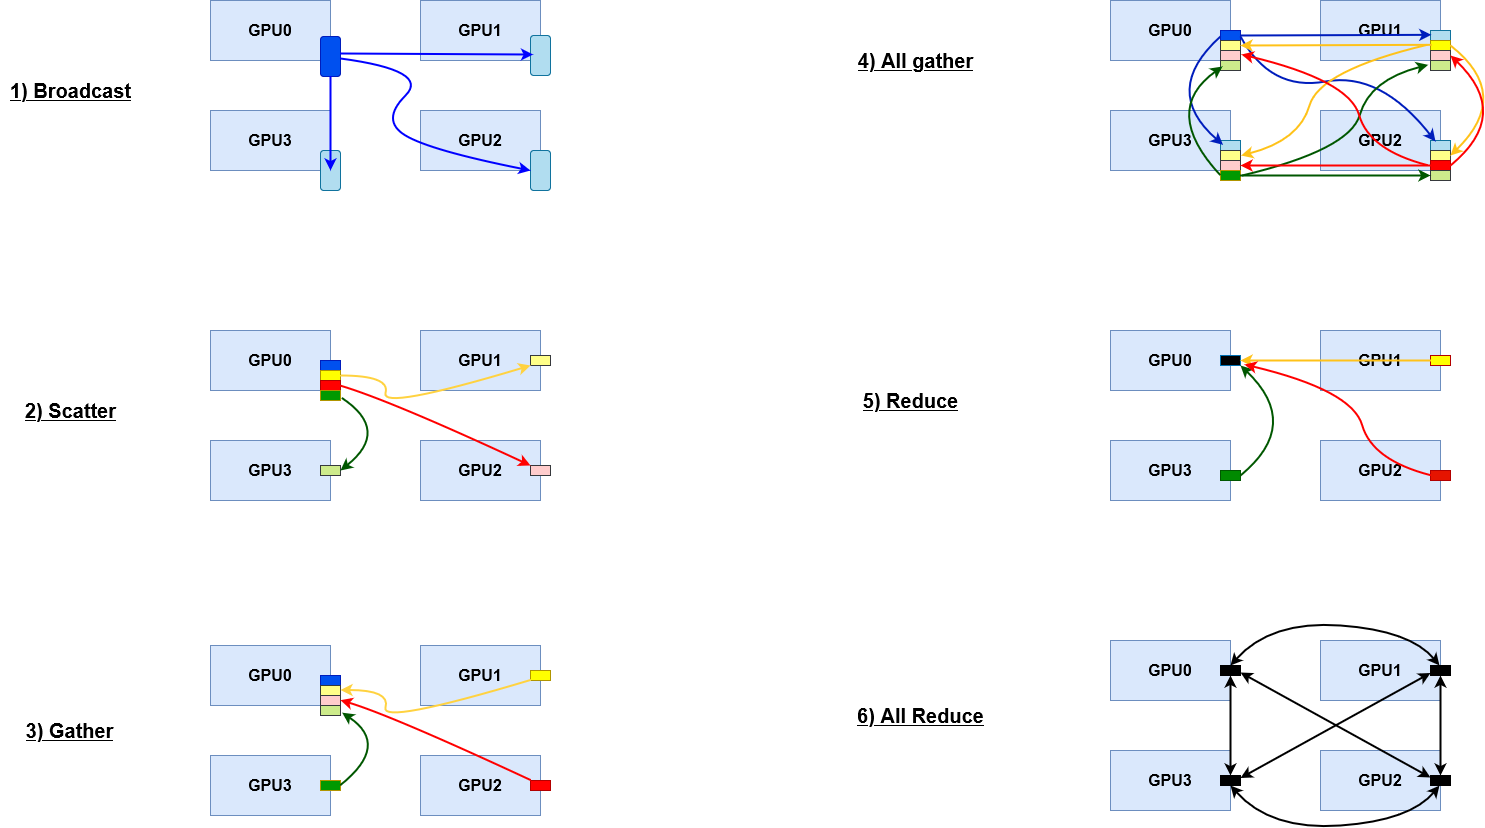
\includegraphics[width=0.7\linewidth]{images/2022-09-07-15-00-16.png}
  \caption{NVIDIA NCCL primitives (credit: https://images.nvidia.com/events/sc15/pdfs/NCCL-Woolley.pdf)}
\end{figure}
\FloatBarrier

All of these said, let's go back to PyTorch and spend some time writing distributed applications!

\subsection{Distributed applications in PyTorch}
If the reader wants to focus on writing distributed Machine Learning models, this section can be skipped. We will here hide the choice of backend behind PyTorch to study some basic communication applications. As seen previously, each backend provides different primitives and thus we have to be careful when using the PyTorch distributed abstraction. The chart below shows which backend supports which method: feel free to refer to it later!

\[\begin{array}{l|ll|ll|ll}
  \text{Backend} & \text{\lstinline{gloo}} & & \text{\lstinline{mpi}} & & \text{\lstinline{nccl}} \\
  \hline\hline
  \text{Device} & \text{CPU} & \text{\GLS{GPU}} & \text{CPU} & \text{\GLS{GPU}} & \text{CPU} & \text{\GLS{GPU}} \\
  \hline
  \text{send} & \checkmark & \chi & \checkmark & \checkmark & \chi & \checkmark \\
  \text{recv} & \checkmark & \chi & \checkmark & \checkmark & \chi & \checkmark \\
  \text{broadcast} & \checkmark & \checkmark & \checkmark & \checkmark & \chi & \checkmark \\
  \text{all\_reduce} & \checkmark & \checkmark & \checkmark & \checkmark & \chi & \checkmark \\
  \text{reduce} & \checkmark & \chi & \checkmark & \checkmark & \chi & \checkmark \\
  \text{all\_gather} & \checkmark & \chi & \checkmark & \checkmark & \chi & \checkmark \\
  \text{gather} & \checkmark & \chi & \checkmark & \checkmark & \chi & \checkmark \\
  \text{scatter} & \checkmark & \chi & \checkmark & \checkmark & \chi & \chi \\
  \text{reduce\_scatter} & \chi & \chi & \chi & \chi & \chi & \checkmark \\
  \text{all\_to\_all} & \chi & \chi & \checkmark & \checkmark & \chi & \checkmark \\
  \text{barrier} & \checkmark & \chi & \checkmark & \checkmark & \chi & \checkmark
\end{array}\]

\subsubsection{Other differences between the backends}
Gloo is considered as a good backend for development purposes: it is included in the pre-compiled PyTorch binaries and works on Linux, Windows and macOS. However, its implementation of the collective operations for CUDA tensors is not as optimized as the ones provided by NCCL. In the example below, we will use this backend, unless stated otherwise. Note that the examples work the same with other backends due to the abstraction.

NCCL is included in the pre-built binaries with CUDA support, and offers the best performance with CUDA tensors. It can however be a bit more tricky to setup depending on one's installation.

Finally, MPI is \textit{the} standardized backend. Several implementations exist and each of them is optimized for different purposes. The major issue is that PyTorch binaries cannot include an MPI implementation, and so the user has to compile it by hand. If interested, the PyTorch documentation has a \href{https://pytorch.org/tutorials/intermediate/dist_tuto.html#communication-backends}{page} indicating how to build PyTorch with MPI.

\subsubsection{Generic setup code}
While processes using \lstinline{torch.multiprocessing} are restricted to be executed on the same machine, the \lstinline{torch.distributed} package uses the different communication backends to allow multiple machines (nodes) to inter-communicate. The  code shown below is one example of how one can set up his distributed environment: note that it will in the end depends on the developers and the project.

\paragraph{Initiating the processes}
We will create a \lstinline{run} method where we write the distributed function. This function is then passed as an argument to the function initiating all processes:

\begin{lstlisting}[language=Python]
def init_process(rank, size, func, backend):
  os.environ['MASTER_ADDR'] = '192.168.1.10' # IP address of master node
  os.environ['MASTER_PORT'] = '29500' # Port of master node
  # Processes share their locations to allow communication
  dist.init_process_group(backend, rank=rank, world_size=size)
  func(rank, size)
\end{lstlisting}

The master node is the one that hosts the process with rank 0. We will dive deeper in the \lstinline{init_process_group} function in the next section when we'll learn how to use the \lstinline{distributedDataParallel} package.

\paragraph{Generating and starting the processes}
\begin{lstlisting}[language=Python]
if __name__ == '__main__':
  size = 2 # World size
  processes = [] # We keep track of our processes
  mp.set_start_method("spawn")
  # Generate a process for each rank (from 0 to size - 1)
  for rank in range(size):
      # Using the Gloo backend
      p = mp.Process(target=init_process, args=(rank, size, run, "gloo"))
      p.start()
      processes.append(p)

  for p in processes:
      p.join()
\end{lstlisting}

The \lstinline{torch.multiprocessing.Process} class follows the API of the Python \lstinline{threading.Thread}. We create it giving the target function and the arguments we want to send to this function.

\subsubsection{Point-to-Point communication}
Point-to-Point communication consists of transferring data from one process to another. Two groups of methods are available, that is the blocking ones and the immediate (non-blocking) ones. In the case of the blocking functions, both processes stop and wait until the communication is completed:

\begin{lstlisting}[language=Python]
def run(rank, size):
  tensor = torch.zeros((2, 2))
  if rank == 0:
      tensor += 1
      # Send the tensor to process 1
      dist.send(tensor=tensor, dst=1)
  else:
      # Receive tensor from process 0
      dist.recv(tensor=tensor, src=0)
  print('Rank ', rank, ' has data ', tensor[0])
\end{lstlisting}
Note how the tensor for the process 1 is never changed in the code it has access to! However, the result shows that it correctly received the modified tensor:
\begin{lstlisting}
Rank  1  has data  tensor([1., 1.])
Rank  0  has data  tensor([1., 1.])
\end{lstlisting}
Also, the destination process \lstinline{dst} is specified in the \lstinline{send} method, while the source process \lstinline{src} is specified in the \lstinline{recv} function.

In the case of non-blocking immediate functions, the programs continues its execution and the methods return a special object \lstinline{Work} on which we choose to call the \lstinline{wait} once we want to use it. Be careful when using immediate functions: modifying the tensor during the communication will result in undefined behaviour!

\begin{lstlisting}[language=Python]
def run(rank, size):
  tensor = torch.zeros((2, 2))
  req = None
  if rank == 0:
      tensor += 1
      # Send the tensor to process 1
      req = dist.isend(tensor=tensor, dst=1)
  else:
      # Receive tensor from process 0
      req = dist.irecv(tensor=tensor, src=0)
  req.wait()
  print('Rank ', rank, ' has data ', tensor[0])
\end{lstlisting}

We get the same result as above. The \lstinline{req} object is defined as \lstinline{None} for all processes and then assigned specifically.

\subsubsection{Collective communication}
As we saw, Point-to-Point communication specifies both a sender and a receiver. Collective communication allows for communication across all processes that are inside the same group (in MPI, we talked about a communicator). For example, we can create the group containing both process 0 and 1:
\begin{lstlisting}[language=Python]
group = dist.new_group([0, 1])
\end{lstlisting}
Exactly like in MPI, the default group consists of the whole world. PyTorch implements a total of 6 collectives (i.e. communicative operations). They are listed here under, but one can find more details about them in the section about the backends:
\begin{itemize}[noitemsep]
  \item \lstinline{dist.broadcast(tensor, src, group)}: copies \lstinline{tensor} from \lstinline{src} to all processes
  \item \lstinline{dist.reduce(tensor, dst, op, group)}: applies \lstinline{op} to every \lstinline{tensor} and stores the result in \lstinline{dst}
  \item \lstinline{dist.all_reduce(tensor, op, group)}: same as reduce, with the result stored in all processes
  \item \lstinline{dist.scatter(tensor, scatter_list, src, group)}: copies the \(i\)-th tensor \lstinline{scatter_list[i]} to the \(i\)-th process
  \item \lstinline{dist.gather(tensor, gather_list, dst, group)}: copies \lstinline{tensor} from all processes in \lstinline{dst}
  \item \lstinline{dist.all_gather(tensor_list, tensor, group)}: copies \lstinline{tensor} from all processes to \lstinline{tensor_list}, on all processes
  \item \lstinline{dist.barrier(group)}: blocks all processes in \lstinline{group} until each one has entered this function
\end{itemize}

\paragraph{A note on the reduce operations}
PyTorch implements 4 type of reduce operations, that are stored in the \lstinline{dist.ReduceOp} object:
\begin{itemize}[noitemsep]
  \item \lstinline{dist.ReduceOp.SUM}
  \item \lstinline{dist.ReduceOp.PRODUCT}
  \item \lstinline{dist.ReduceOp.MAX}
  \item \lstinline{dist.ReduceOp.MIN}
\end{itemize}

\paragraph{Example with scattering}
Let's get ahead and write an example for the \lstinline{dist.scatter} collective. We first create a group and initialize a tensor. The scatter methods takes a tensor as its first parameter: this is where the scattered tensor will be stored. The second parameters \lstinline{scatter_list} must only be specified by the process that sends the tensors. The others processes must have \lstinline{None} (default value) for this parameter. The third is the source process and the last parameter is the communication group.

\begin{lstlisting}[language=Python]
def run(rank, size):
  group = dist.new_group([0, 1])
  tensor = torch.zeros(2)
  if rank == 0:
      scatter_tensors = [torch.tensor([0., 1.]), torch.tensor([2., 3.])]
      dist.scatter(tensor, scatter_tensors, src=0, group=group)
  else:
      dist.scatter(tensor, None, src=0, group=group)
  print('Rank ', rank, ' has data ', tensor)
\end{lstlisting}
We thus get the expected result, i.e.:
\begin{lstlisting}
Rank  0  has data  tensor([0., 1.])
Rank  1  has data  tensor([2., 3.])
\end{lstlisting}

\paragraph{Example with reducing}
One more example for the road! This time, let's write a very simple reducing operation. We set up our group, generate some tensors using the rank and run a \lstinline{dist.reduce} collective, using the \lstinline{dist.ReduceOp.PRODUCT} operation:
\begin{lstlisting}[language=Python]
def run(rank, size):
  group = dist.new_group([0, 1])
  tensor = torch.tensor([rank + 1, rank + 10])
  dist.reduce(tensor, dst=0, op=dist.ReduceOp.PRODUCT, group=group)
  print('Rank ', rank, ' has data ', tensor)
\end{lstlisting}
The process with rank 1 shouldn't see its tensor being changed, but the root process should have the multiplication of all tensors. This is indeed what we observe:
\begin{lstlisting}
Rank  1  has data  tensor([2, 11])
Rank  0  has data  tensor([2, 110])
\end{lstlisting}
The rank 0 process gets the tensor \([1, 10]\cdot [2, 11]\) where \(\cdot \) represents an element-wise product.

\subsection{The \texorpdfstring{\lstinline{distributedDataParallel}}{distributedDataParallel} module}
Now that we explored the basics of collective communication with PyTorch, let's head back into our goal: parallelize Machine Learning models. For this, we need to explore the \lstinline{distributedDataParellel} package.

The most important function in this package is the constructor itself. This container parallelizes the application of the given module by splitting the input across the specified devices by chunking in the batch dimension. The module is replicated on each machine, and every replica handles a portion of the input. During the backwards pass, gradients from each node are averaged. This means that the batch size should be larger than the number of \GLS{GPU}s used locally.

\begin{lstlisting}[language=Python]
from torch.nn.parallel import DistributedDataParallel as DDP
ddp_model = DDP(model, device_ids=[rank])
\end{lstlisting}

\subsubsection{Torch \texorpdfstring{\lstinline{multiprocessing}}{multiprocessing} package}
The \lstinline{torch.multiprocessing} package wraps the native \lstinline{multiprocessing} module of Python. I won't enter into details here, instead I want to introduce a very important function, the \lstinline{spawn} method:
\begin{lstlisting}[language=Python]
torch.multiprocessing.spawn(func, args=(), nprocs, join, daemon, start_method='spawn')
\end{lstlisting}
As its name entails, this method \textit{spawns} (i.e. creates or generates) \lstinline{nprocs} processes that each run the given function \lstinline{func} with the arguments \lstinline{args}. The function is called as \lstinline{func(i, *args)}, where \lstinline{i} is the index of the process (sounds like the rank, doesn't it?) and where the \lstinline{args} tuple is deconstructed to give each element as a parameter directly. The \lstinline{join} argument allows to perform a blocking join on all processes. If set to \lstinline{false}, a \lstinline{ProcessContext} is returned by the method and the joining has to be done manually. Note that the last argument \lstinline{start_method} is deprecated, you should not change its default value.

\subsubsection{Initiating the group}
Each process has to know which distributed process group it is a part of. For that, a good practice is to create a setup function to prepare the environment and initiate the group. This is the same function as \lstinline{init_process} in the section about distributed applications. This function is run for each process. For instance:
\begin{lstlisting}[language=Python]
def setup(rank, world_size, backend):
  os.environ['MASTER_ADDR'] = '192.168.1.10'
  os.environ['MASTER_PORT'] = '12355'
  dist.init_process_group(backend, rank=rank, world_size=world_size)
\end{lstlisting}
This very simple example sets the master's IP address and port, and prepares the process giving it the backend used, its rank and the world size.
The method used is the following:
\begin{lstlisting}[language=Python]
torch.distributed.init_process_group(backend, init_method, timeout, world_size, rank, store, group_name, pg_options)
\end{lstlisting}
In the example above, we initialize a process group explicitly, but it is also possible to specify an \lstinline{init_method} which indicates how to discover the peers. The \lstinline{store} parameter, mutually exclusive with the \lstinline{init_method} serves as the key/value store accessible to all workers and is used to interchange connection and/or address information.

\paragraph{Using a shared file system}
Sometimes, it is useful to allow all processes to access a shared file system: they will open the file, write their information and then wait for every processes to complete the same steps. The file system must support locking through \lstinline{fcntl} to avoid race conditions.

\begin{lstlisting}[language=Python]
dist.init_process_group(init_method='file:///mnt/nfs/sharedfile', rank=rank, world_size=size)
\end{lstlisting}

\paragraph{Using TCP}
It is also possible to directly indicate the IP address of the root node (the one owning the process with rank 0) and the port number. All workers (the non-root nodes) will be able to connect to the root process (rank 0) and exchange their information on how to reach one another.

\begin{lstlisting}[language=Python]
dist.init_process_group(init_method='tcp://192.168.1.10:23456', rank=rank, world_size=size)
\end{lstlisting}

\subsubsection{Destroying the group}
At the end of the training, it is good practice to destroy the process group and de-initialize the distributed package:
\begin{lstlisting}[language=Python]
def cleanup():
  dist.destroy_process_group()
\end{lstlisting}

\subsubsection{Complete (simple) example}
Let's go through a complete example of a model that uses the \lstinline{DistributedDataParallel} package:
\begin{lstlisting}[language=Python]
# Imports and hyperparameters ...

def setup(rank, world_size):
    os.environ['MASTER_ADDR'] = 'localhost'
    os.environ['MASTER_PORT'] = '12355'

    dist.init_process_group("gloo", rank=rank, world_size=world_size)

def cleanup():
    dist.destroy_process_group()

class Net(nn.Module):
    # Model ...

def main(rank, world_size):
    setup(rank, world_size)

    model = Net().cuda(rank)
    ddp_model = DDP(model, device_ids=[rank])
    torch.cuda.set_device(rank)

    train_dataset = datasets.MNIST('./data/', download=True, train=True, transform=transform)
    train_sampler = torch.utils.data.distributed.DistributedSampler(train_dataset, num_replicas=world_size, rank=rank, shuffle=False)
    train_loader = torch.utils.data.DataLoader(dataset=train_dataset, batch_size=batch_size, shuffle=False, pin_memory=True, sampler=train_sampler)

    criterion = nn.NLLLoss()
    optimizer = optim.SGD(ddp_model.parameters(), lr=learning_rate)

    for _ in range(epochs):
        # Training process ...
        # Don't forget here to move the tensors to the right process using the .cuda(rank) method!

    cleanup()

def run(fn, world_size):
    mp.spawn(fn, args=(world_size,), nprocs=world_size, join=True)

if __name__ == "__main__":
    world_size = torch.cuda.device_count()
    run(main, world_size)
\end{lstlisting}

\subsection{The ZeRO memory optimizer}
ZeRO is a breakthrough optimization technology developed by Microsoft for large-scale distributed deep learning. It destroyed the competition by going 3 to 5 times faster, allowing the possibility to efficiently train models with trillions of parameters. It is a part of DeepSpeed, but we will talk about that one a bit later.

ZeRO partitions the model states (i.e. parameters, gradients and optimizer state) across all processes instead of replicating them, thus removing the memory redundancies. It introduced a dynamic communication schedule during training that allows to retain the computational precision and communication volume of data parallelism. Using the combined optimizer state partitioning, gradient partitioning and parameter partitioning, ZeRO claims to yield a 64x memory reduction compared to classical methods.

\subsection{Let's simplify our work with DeepSpeed}
We already began hiding the details of the framework away, using the integrated distributed methods from PyTorch. Let's now go deeper into this by adding a layer: DeepSpeed. DeepSpeed is an optimization software, created by Microsoft in 2020 along with ZeRO, that enables huge scaling and speed increase for deep learning models. It is quite easy to setup, especially with an existing PyTorch DistributedDataParallel model.

Let's begin with an example of a simple model using DeepSpeed that I will break down quickly here before diving deeper into the functions and the numerous parameters in the following subsections.

\begin{lstlisting}[language=Python]
# Usual imports ...
import deepspeed

def add_argument():
    parser = argparse.ArgumentParser(description='CIFAR')
    parser.add_argument('--with_cuda',
                        default=False,
                        action='store_true')
    # Other arguments ...
    # Include DeepSpeed configuration arguments
    parser = deepspeed.add_config_arguments(parser)
    args = parser.parse_args()
    return args

deepspeed.init_distributed(dist_backend="gloo")

# Transform ...

if torch.distributed.get_rank() != 0:
    # might be downloading cifar data, let rank 0 download first
    torch.distributed.barrier()

# Use classical DataLoader and CIFAR10 dataset ...

if torch.distributed.get_rank() == 0:
    # cifar data is downloaded, indicate other ranks can proceed
    torch.distributed.barrier()

classes = ('plane', 'car', 'bird', 'cat', 'deer', 'dog', 'frog', 'horse', 'ship', 'truck')

args = add_argument()

class Net(nn.Module):
    def __init__(self):
        # Create the model ...

    def forward(self, x):
        # ... and the forward method as usual ...

net = Net()
net.requires_grad_(False)

model_engine, optimizer, trainloader, __ = deepspeed.initialize(args=args, model=net, model_parameters=net.parameters(), training_data=trainset)

criterion = nn.CrossEntropyLoss()

for epoch in range(args.epochs):
    for i, data in enumerate(trainloader):
        inputs, labels = data[0].to(model_engine.local_rank), data[1].to(model_engine.local_rank)
        outputs = model_engine(inputs)
        loss = criterion(outputs, labels)

        model_engine.backward(loss)
        model_engine.step()
\end{lstlisting}
We can see a few changes compared to the PyTorch way of doing things.
\begin{itemize}
  \item The \lstinline{deepspeed.init_distributed()} method is very similar to the \lstinline{torch.distributed.init_process_group()} and does mostly the same job. Note that the default backend is NCCL. It is not necessary to use this function if no modification to the distributed setup are made, as the next function we'll see, \lstinline{deepspeed.initialize()} will automatically initialize the distributed environnement.
  \item The \lstinline{deepspeed.initialize()} method is the most important: it ensures that all of the necessary setup required is done approprietely (and almost invisibly from the user). It can create and manage not only the model, but also the optimizer, the data loader and the learning rate schedulder (we'll talk much more about these later).
  \begin{lstlisting}[language=Python]
model_engine, optimizer, _, _ = deepspeed.initialize(args=args, model=model, model_parameters=model.parameters())
  \end{lstlisting}
\end{itemize}
One quite clever trick used in this example is the usage of the \lstinline{torch.distributed.barrier()} method, that blocks a processus from operating further until all processes received the method. Here, we use it to download all the CIFAR10 data on the root node (with the root process) without having the other processes try to obtain it. Once the data is downloaded, we call the barrier method on the node 0 as well, liberating every node and allowing the program to continue.

\subsubsection{What DeepSpeed is actually doing}
DeepSpeed is abstracting most of the work away from the developer, but what "work" are we talking about? The answer is: pretty much everything. As stated by the official documentation, "DeepSpeed automatically performs the necessary operations required for distributed data parallel training, in mixed precision, with a pre-defined learning rate scheduler". It ensures that gradients are averaged across all data parallel processes, scales the loss to avoid loss in the gradients and handles the \lstinline{step()} function with a learning rate scheduler.

\subsubsection{The DeepSpeed configuration}
Most of the configuration for DeepSpeed is located in a file usually called \lstinline{ds_config.json}. We won't discuss \textit{all} of the configuration parameters here (as there are \textit{a lot} of them). Please refer to the official documentation if needed (\href{https://www.deepspeed.ai/docs/config-json/}{DeepSpeed configuration documentation}).

\subsubsection{Launching a DeepSpeed model}
While not mandatory per se, it is good practice to create a runnable file to launch a model, especially when using a framework such as DeepSpeed. For example, a file called \lstinline{run_ds.sh} contains the following code:
\begin{lstlisting}[language=bash]
NUM_NODES=1
NUM_\GLS{GPU}S=2

deepspeed --num_nodes=${NUM_NODES} --num_\GLS{GPU}s=${NUM_\GLS{GPU}S} deepspeed_model.py \
	--deepspeed \
	--deepspeed_config ds_config.json
\end{lstlisting}
This is a very straightforward bash file calling \lstinline{deepspeed} with only two parameters, which are the number of nodes and the number of \GLS{GPU}s. We must always indicate the location of the configuration file as well.

\clearpage
\printglossaries

\clearpage
\section{Annex}
In this section, I will write and briefly describe codes that can be useful in order to attain a better understanding of the backends and the parallelization in PyTorch. I recommend the reader to take some time to experiment and play with them.

It also contains a few brief tutorials for setting one's system up.

\subsection{MPI}
\subsubsection{Simple send-receive peer-to-peer exchange}
This first example consists of a simple exchange from a sender to a receiver. We send a number across the devices: rank 0 (root) is the sender and rank 1 will receive and print the result.

\begin{lstlisting}[language=C]
#include <mpi.h>
#include <stdio.h>

int main(int argc, char **argv) {
    MPI_Init(NULL, NULL);
    int rank;
    MPI_Comm_rank(MPI_COMM_WORLD, &rank);
    int size;
    MPI_Comm_size(MPI_COMM_WORLD, &size);

    int number;
    if(rank == 0) {
        number = 43523;
        MPI_Send(&number, 1, MPI_INT, 1, 0, MPI_COMM_WORLD);
    } else if(rank == 1) {
        MPI_Recv(&number, 1, MPI_INT, 0, 0, MPI_COMM_WORLD, MPI_STATUS_IGNORE);
        printf("Process 1 received number %d from process 0\n", number);
    }
    MPI_Finalize();
}
\end{lstlisting}

It is important here to note that the node with rank 1 has not seen what the number is initialized to: one must be careful about what each process knows from the code itself or from what it receives from other nodes.

\subsubsection{Approximating \texorpdfstring{$\pi$}{pi} using multiple processes}
Let's go through a quite fun example. We are here trying to approximate \(\pi\) using the Taylor series expansion for \(\arctan(1)\), using the fact that \(\pi=4\cdot \frac{\pi}{4}=4\cdot \arctan(1)\).
\[\arctan(1)=\sum_{n=0}^{\infty} \frac{(-1)^n}{2n+1}\]

The idea is that each process will compute one element of this sum. We then use \lstinline{MPI_Reduce} with the sum operation to compute \(\frac{\pi}{4}\) and multiply it by 4. The result is sent to the root process defined in the head of the code, and the root process is asked to print the result.

\begin{lstlisting}[language=C]
#include <stdio.h>
#include <stdlib.h>
#include <mpi.h>
#include <math.h>

#define ROOT 0

double taylor(const int i, const double x, const double a) {
    int sign = pow(-1, i);
    double num = pow(x, 2 * i + 1);
    double den = a * (2 * i + 1);
    return (sign * num / den);
}

int main(int argc, char *argv[]) {
    int nodes, rank;
    double* partial;
    double res;
    double total = 0;

    MPI_Init(&argc, &argv);
    MPI_Comm_size(MPI_COMM_WORLD, &nodes);
    MPI_Comm_rank(MPI_COMM_WORLD, &rank);

    res = taylor(rank, 1, 1);
    printf("rank=%d total=%f\n", rank, res);

    MPI_Reduce(&res, &total, 1, MPI_DOUBLE, MPI_SUM, ROOT, MPI_COMM_WORLD);

    if(rank == ROOT)
        printf("Total is = %f\n", 4*total);

    MPI_Finalize();
}
\end{lstlisting}

\subsection{NCCL}
% TODO: NCCL code is not working on my computer (GPUs crashing)

\subsection{Build PyTorch with MPI}
% TODO

\subsection{Full simple DeepSpeed example}
Here under is the full example about DeepSpeed that is presented early in the DeepSpeed section. The most important parts of code are already described in the mentioned section, please refer to it for more information.
\begin{lstlisting}[language=Python]
import torch
import torchvision
import torchvision.transforms as transforms
import argparse
import torch.nn as nn
import torch.nn.functional as F
import deepspeed

def add_argument():
    parser = argparse.ArgumentParser(description='CIFAR')
    parser.add_argument('--with_cuda',
                        default=False,
                        action='store_true',
                        help='use CPU in case there\'s no GPU support')
    parser.add_argument('-b',
                        '--batch_size',
                        default=32,
                        type=int,
                        help='mini-batch size (default: 32)')
    parser.add_argument('-e',
                        '--epochs',
                        default=30,
                        type=int,
                        help='number of total epochs (default: 30)')
    parser.add_argument('--local_rank',
                        type=int,
                        default=-1,
                        help='local rank passed from distributed launcher')
    parser.add_argument('--log-interval',
                        type=int,
                        default=2000,
                        help="output logging information at a given interval")

    # Include DeepSpeed configuration arguments
    parser = deepspeed.add_config_arguments(parser)
    args = parser.parse_args()
    return args

deepspeed.init_distributed(dist_backend="gloo")

transform = transforms.Compose([
    transforms.ToTensor(),
    transforms.Normalize((0.5, 0.5, 0.5), (0.5, 0.5, 0.5))
])

if torch.distributed.get_rank() != 0:
    # might be downloading cifar data, let rank 0 download first
    torch.distributed.barrier()

trainset = torchvision.datasets.CIFAR10(root='./data',
                                        train=True,
                                        download=True,
                                        transform=transform)

if torch.distributed.get_rank() == 0:
    # cifar data is downloaded, indicate other ranks can proceed
    torch.distributed.barrier()

trainloader = torch.utils.data.DataLoader(trainset,
                                          batch_size=16,
                                          shuffle=True,
                                          num_workers=2)

classes = ('plane', 'car', 'bird', 'cat', 'deer', 'dog', 'frog', 'horse', 'ship', 'truck')

args = add_argument()

class Net(nn.Module):
    def __init__(self):
        super(Net, self).__init__()
        self.conv1 = nn.Conv2d(3, 6, 5)
        self.pool = nn.MaxPool2d(2, 2)
        self.conv2 = nn.Conv2d(6, 16, 5)
        self.fc1 = nn.Linear(16 * 5 * 5, 120)
        self.fc2 = nn.Linear(120, 84)
        self.fc3 = nn.Linear(84, 10)

    def forward(self, x):
        x = self.pool(F.relu(self.conv1(x)))
        x = self.pool(F.relu(self.conv2(x)))
        x = x.view(-1, 16 * 5 * 5)
        x = F.relu(self.fc1(x))
        x = F.relu(self.fc2(x))
        x = self.fc3(x)
        return x

net = Net()
net.requires_grad_(False)

# parameters = filter(lambda p: p.requires_grad, net.parameters())

model_engine, optimizer, trainloader, __ = deepspeed.initialize(args=args, model=net, model_parameters=net.parameters(), training_data=trainset)

fp16 = model_engine.fp16_enabled()
print(f'fp16={fp16}')

criterion = nn.CrossEntropyLoss()

for epoch in range(args.epochs):
    running_loss = 0.0
    for i, data in enumerate(trainloader):
        inputs, labels = data[0].to(model_engine.local_rank), data[1].to(model_engine.local_rank)
        if fp16:
            inputs = inputs.half()
        outputs = model_engine(inputs)
        loss = criterion(outputs, labels)

        model_engine.backward(loss)
        model_engine.step()

        # print statistics
        running_loss += loss.item()
        if i % args.log_interval == (args.log_interval - 1):  # print every log_interval mini-batches
            print('[%d, %5d] loss: %.3f' %  (epoch + 1, i + 1, running_loss / args.log_interval))
            running_loss = 0.0

print('Finished Training')
\end{lstlisting}

\clearpage
\section{Sources}
Work in progress...
\begin{itemize}
    \item \href{https://huggingface.co/docs/transformers/main/en/perf_train_gpu_many#data-parallelism}{Huggingface parallelization}
    \item \href{https://pytorch.org/tutorials/beginner/dist_overview.html}{PyTorch distributed overview}
    \item \href{https://pytorch.org/tutorials/intermediate/ddp_tutorial.html}{PyTorch DDP tutorial}
    \item \href{https://pytorch.org/tutorials/intermediate/dist_tuto.html}{PyTorch distributed tutorial}
    \item \href{https://indico.desy.de/event/12535/contributions/9450/attachments/6466/7452/CL5_MPI_Lecture.pdf}{MPI lesson}
    \item \href{https://images.nvidia.com/events/sc15/pdfs/NCCL-Woolley.pdf}{NVIDIA NCCL introduction slides}
\end{itemize}

\end{document}